\documentclass{beamer}

\usepackage{graphicx}
\usepackage{booktabs}
\usepackage[flushleft]{threeparttable}
\usepackage{amsmath}  % For math symbols
\usepackage[scheme=plain]{ctex}       % 中文支持

\usepackage{graphicx}


\author{Hongming Liang\\  2022201480}
\title{"Community Name" is All You Need?\\ What Feature Really Matters}
\date{2025/06/12}

\begin{document}

\frame{\titlepage}

\begin{frame}{\small Scores}
\begin{scriptsize}
\begin{table}
        \center
        \caption{\scriptsize RMSE for Models}
        \begin{tabular}{ccccc}
            \toprule
            \toprule
            Model & In sample & Out of sample  & Datahub Score \\
            \midrule
            OLS & 467447 & 542005  & 83.209 \\
            RF & - & - & 80.538\\
            XGB & 182028 & 581316 & 82.656\\
            Embedded ANN & -  & - & 82.435\\
            ANN & 298844 & 491192  & 84.764\\
            Ensemble & 301843 & 479520  & 84.857\\
            \bottomrule
        \end{tabular}
\end{table}    
\begin{figure}
    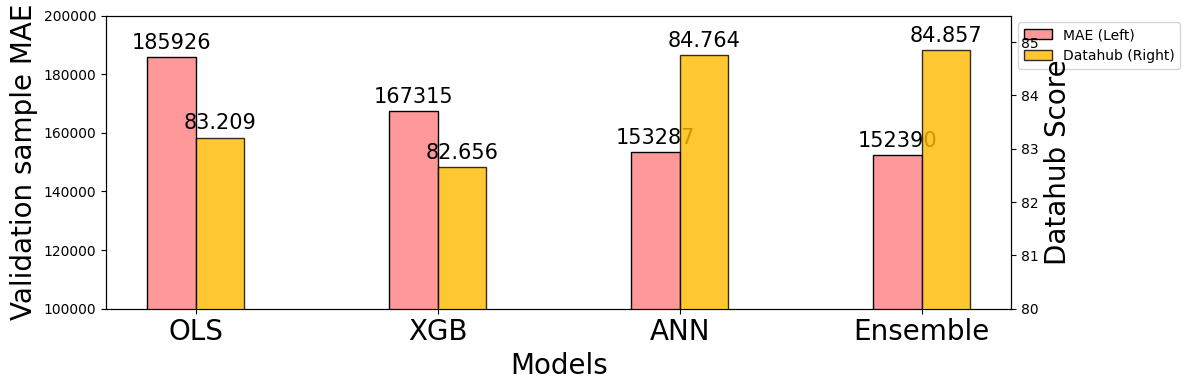
\includegraphics[width=\linewidth]{figure/scores.png}
\end{figure}
\end{scriptsize}
\end{frame}

\begin{frame}{\footnotesize XGB with Optuna. See xgb\_1.ipynb}
\begin{figure}
        \begin{minipage}[t]{0.48\textwidth}
            \center
            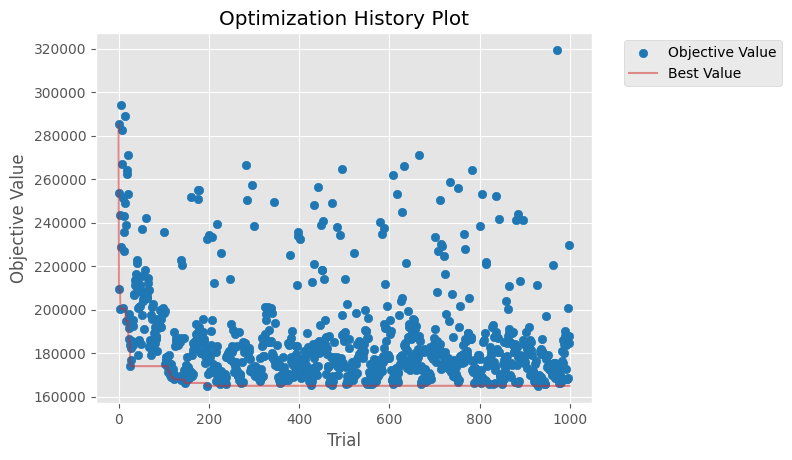
\includegraphics[width=\linewidth]{figure/xgb_1_historyPlot.png}
        \end{minipage}
        \begin{minipage}[t]{0.48\textwidth}
            \center
            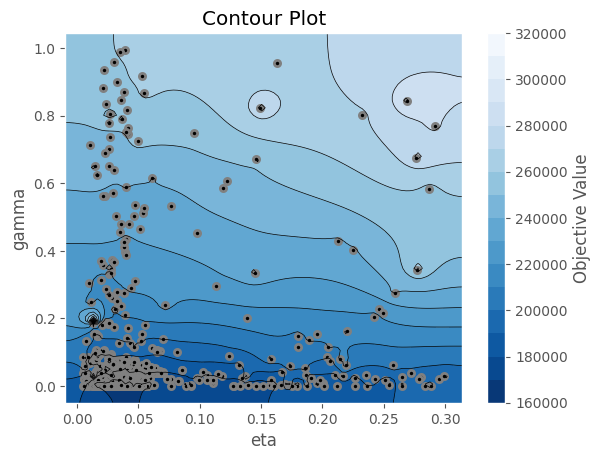
\includegraphics[width=\linewidth]{figure/xgb_1_gamma_eta.png}
        \end{minipage}
    \end{figure}
\begin{figure}
        \begin{minipage}[t]{0.48\textwidth}
            \center
            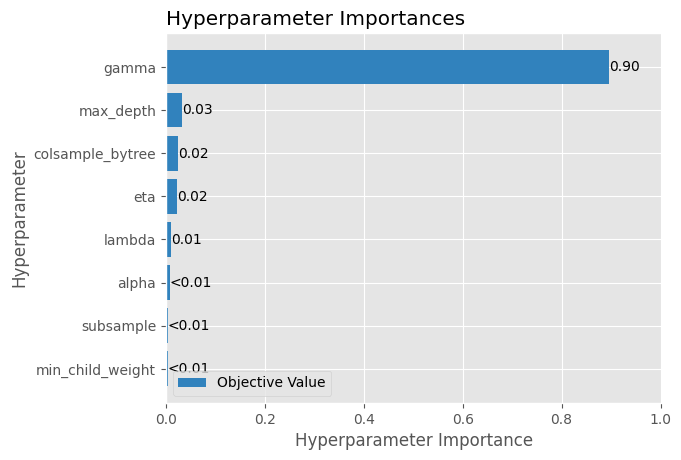
\includegraphics[width=\linewidth]{figure/xgb_1_hyperImportance.png}
        \end{minipage}
        \begin{minipage}[t]{0.48\textwidth}
            \center
            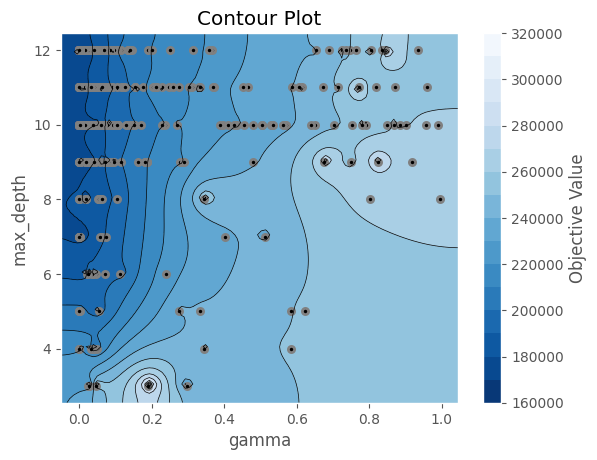
\includegraphics[width=\linewidth]{figure/xgb_1_depth_gamma.png}
        \end{minipage}
    \end{figure}
\end{frame}

\begin{frame}
\begin{itemize}
    \item {\footnotesize XGB with Optuna. See xgb\_2.ipynb}
\end{itemize}
\begin{figure}
        \begin{minipage}[t]{0.48\textwidth}
            \center
            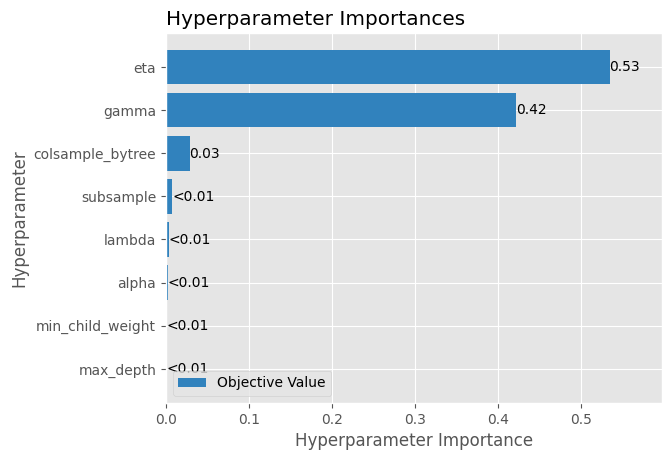
\includegraphics[width=\linewidth]{figure/xgb_2_hyperImportance.png}
        \end{minipage}
        \begin{minipage}[t]{0.48\textwidth}
            \center
            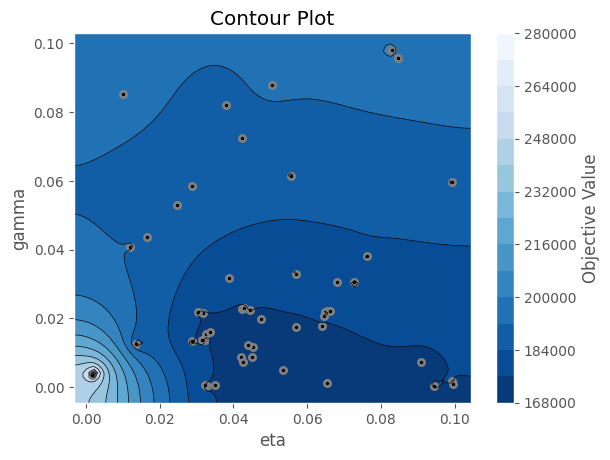
\includegraphics[width=\linewidth]{figure/xgb_2_gamma_eta.png}
        \end{minipage}
    \end{figure}
    \begin{itemize}
        \item {\footnotesize Ann with embedded category feature. See nn\_embbedded.ipynb}
    \end{itemize}
\begin{figure}
    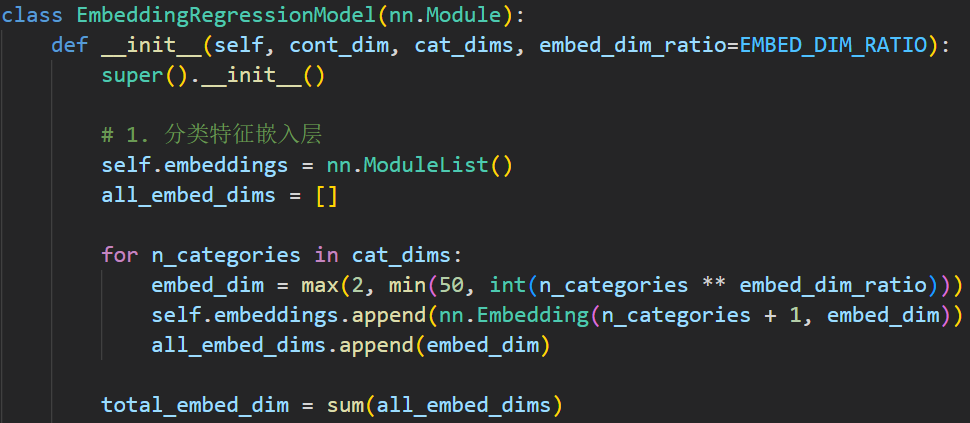
\includegraphics[width=0.8\linewidth]{figure/embed.jpg}
\end{figure}
\end{frame}

\begin{frame}
\begin{figure}
    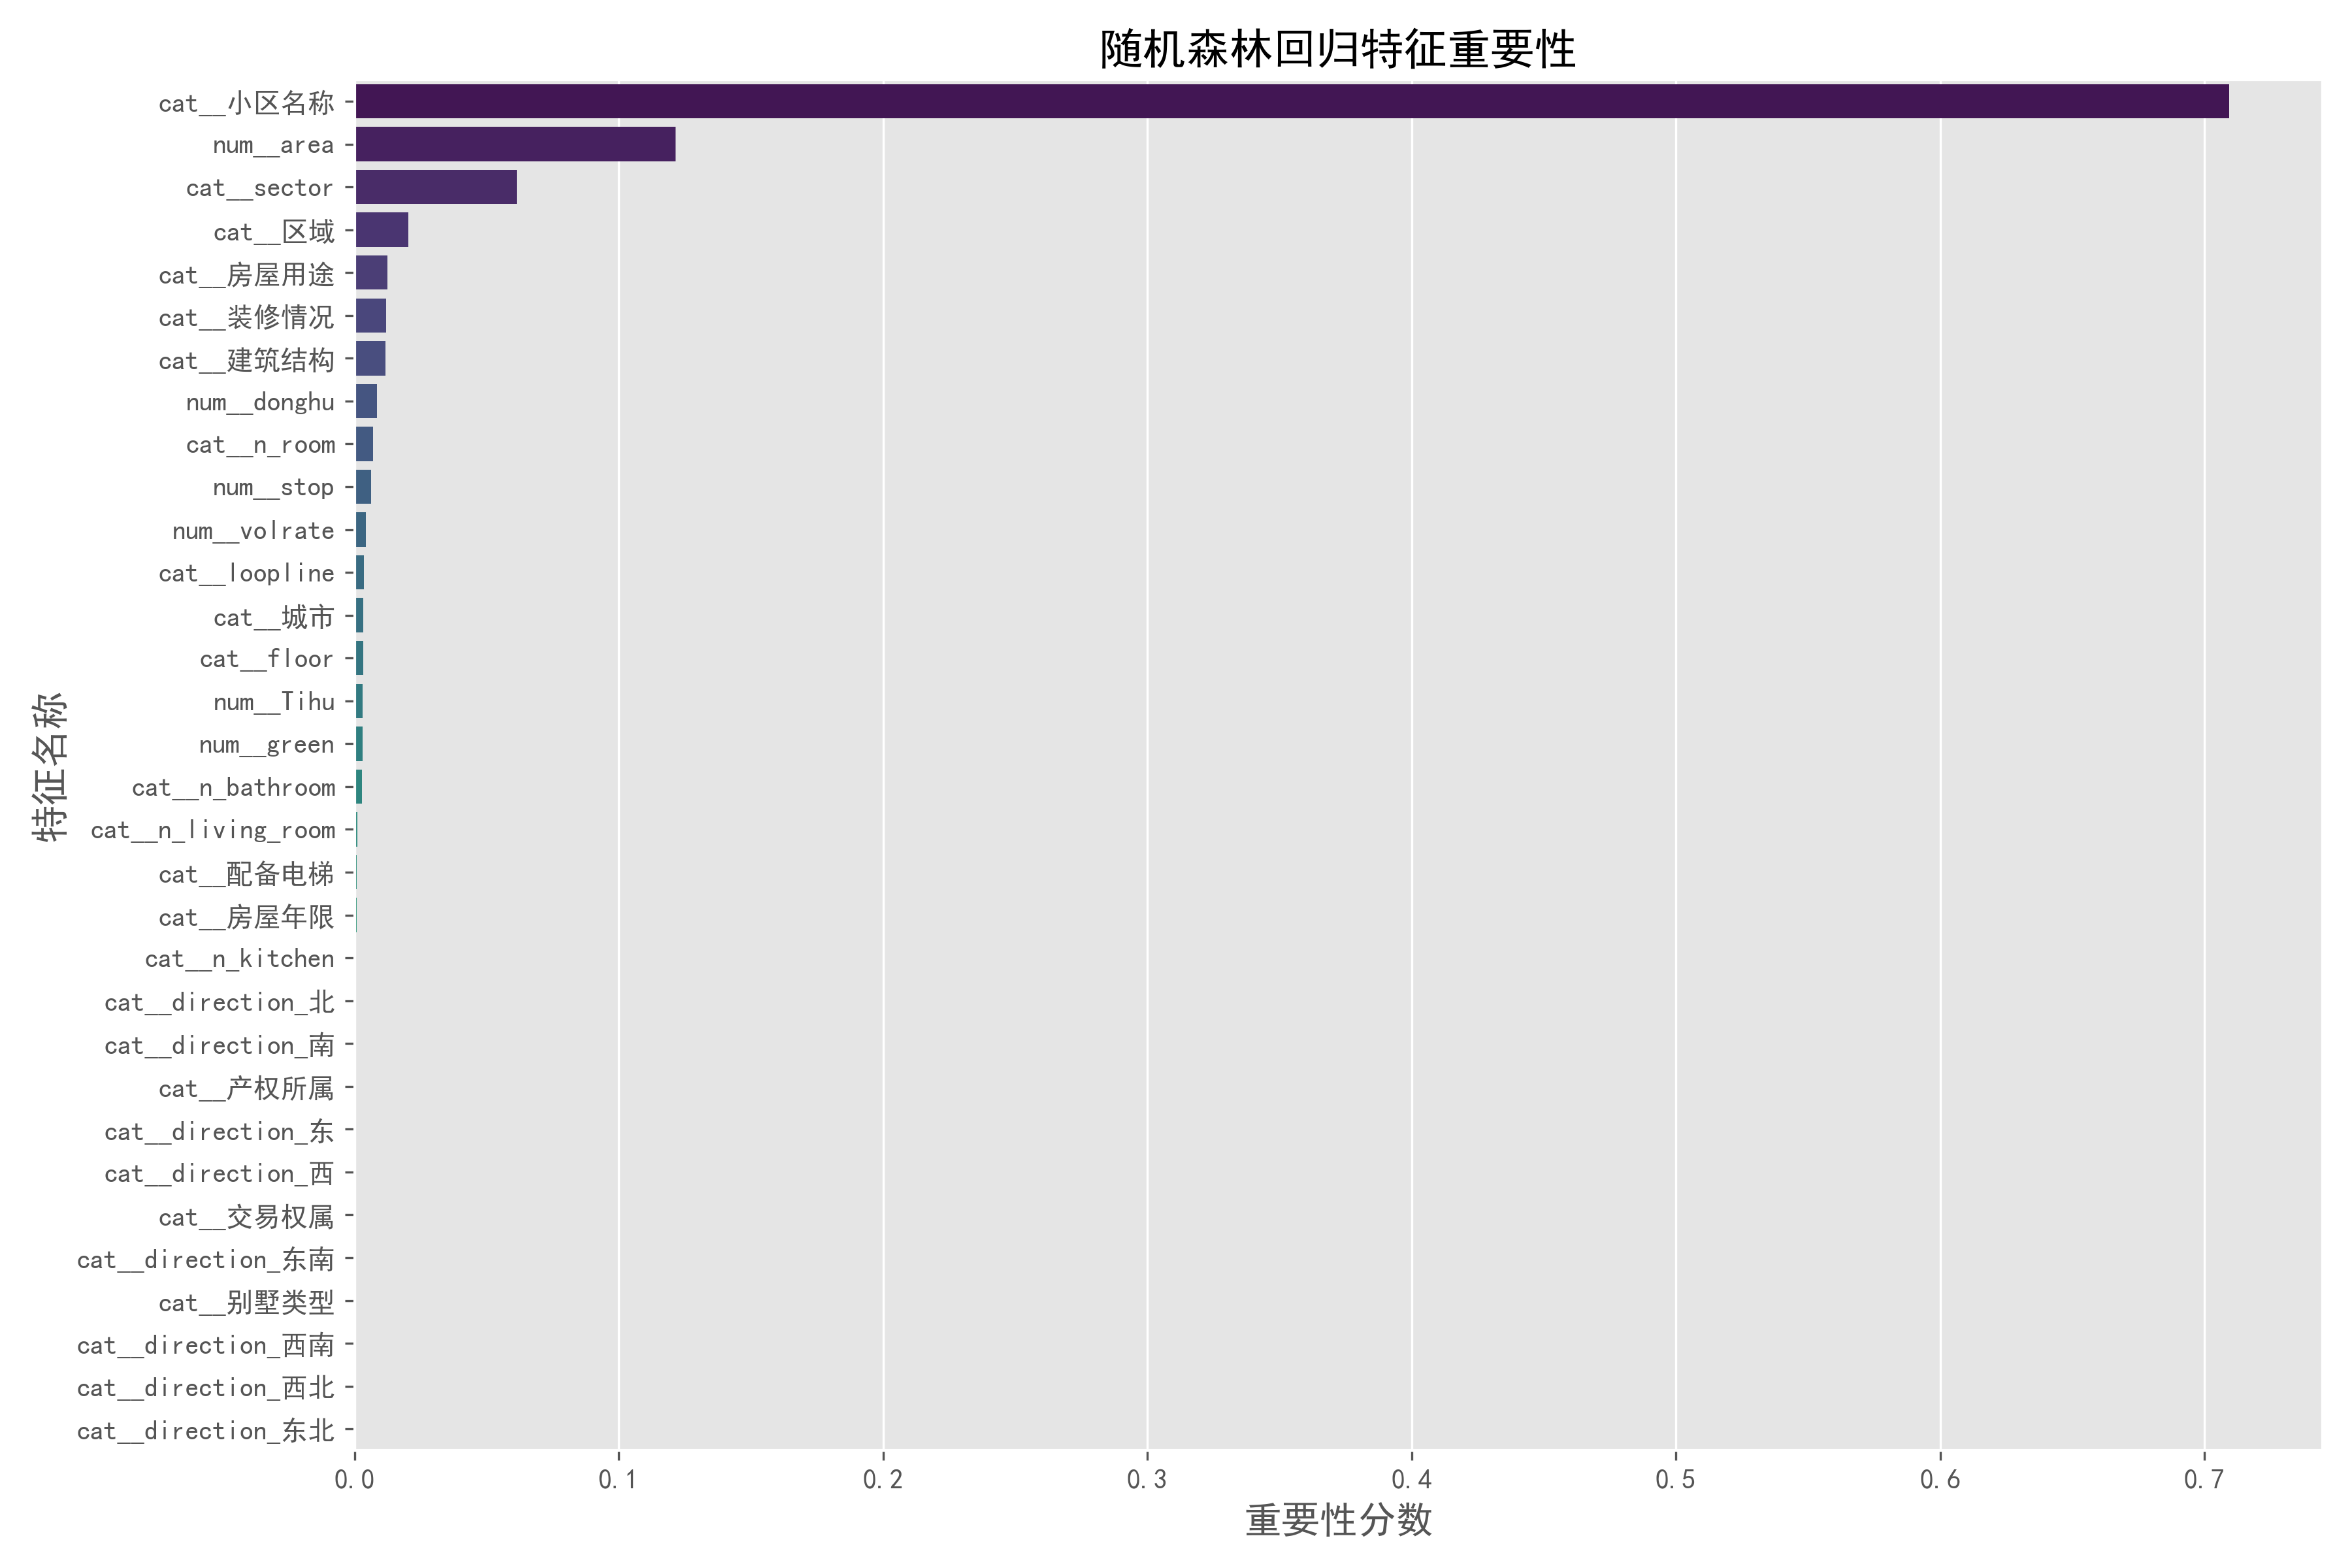
\includegraphics[width=\linewidth]{figure/rf_feature_importance.png}
\end{figure}
\begin{scriptsize}
    \begin{table}
    \center
    \begin{tabular}{cccccc}
        \toprule
        \toprule
        OLS &(1)&(2)&(3)&(4)&(5)\\
        Varible & Area  & (1)+City & (1)+Community & (3)+City+Region & (4)+Sector\\
        \midrule
        Scores & 25.892 & 53.814 & 73.091 & 81.235 & 82.333\\
    \end{tabular}
\end{table}
\end{scriptsize}
\end{frame}

\begin{frame}
    \begin{figure}
        \begin{minipage}[b]{0.28\textwidth}
            {\footnotesize Best Model: ANN\\See ann\_best.ipynb}
            \center
            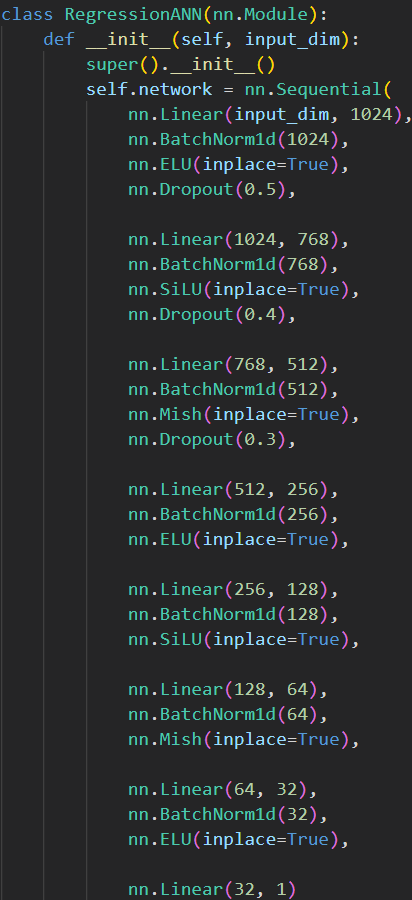
\includegraphics[width=\linewidth]{figure/nn.png}
        \end{minipage}
        \begin{minipage}[b]{0.68\textwidth}
            \begin{figure}
                \center
                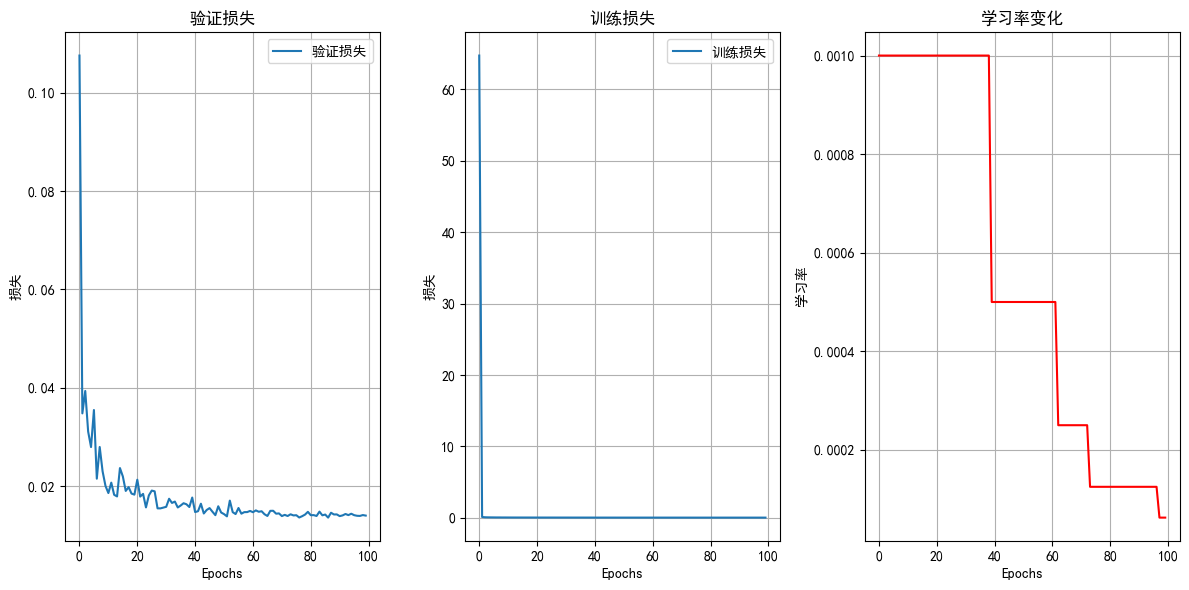
\includegraphics[width=\linewidth]{figure/nn_train.png}
            \end{figure}
            \begin{figure}
                \center
                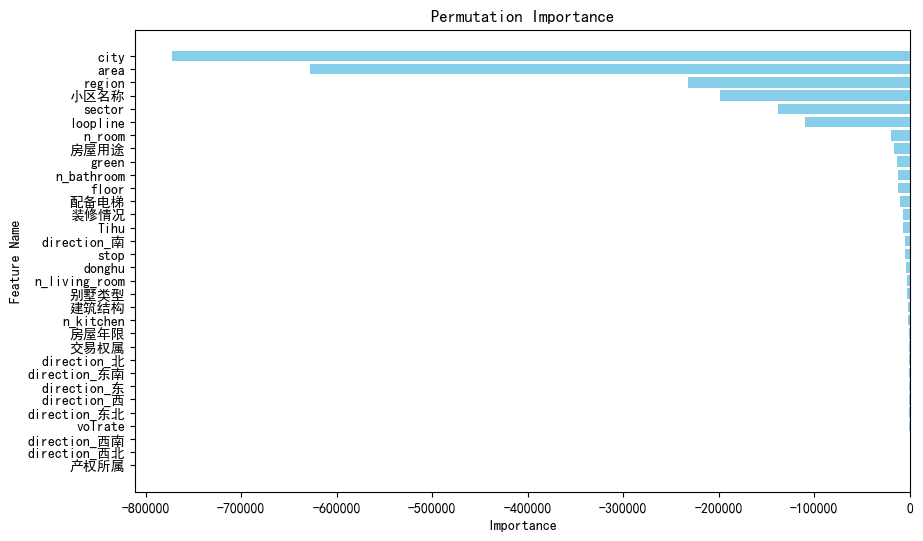
\includegraphics[width=\linewidth]{figure/perin.png}
            \end{figure}
        \end{minipage}
    \end{figure}
\end{frame}

\begin{frame}
    \begin{itemize}
        \item {\small PDP of ANN}
    \end{itemize}
        \begin{minipage}[t]{0.32\textwidth}
            \begin{figure}
                {\tiny Area}
                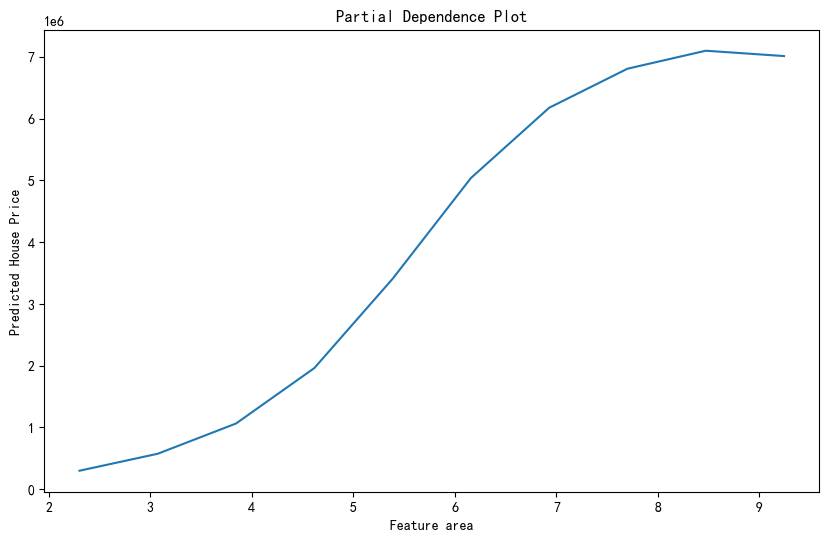
\includegraphics[width=\linewidth]{figure/pdp_area_train.png}
            \end{figure}
            \begin{figure}
                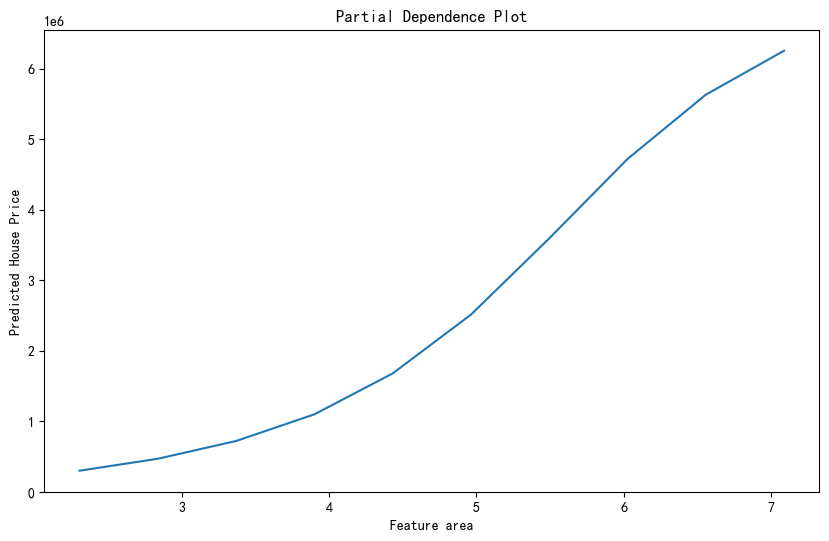
\includegraphics[width=\linewidth]{figure/pdp_area_val.png}
            \end{figure}
        \end{minipage}
        \begin{minipage}[t]{0.32\textwidth}
            \begin{figure}
                {\tiny  绿化率}
                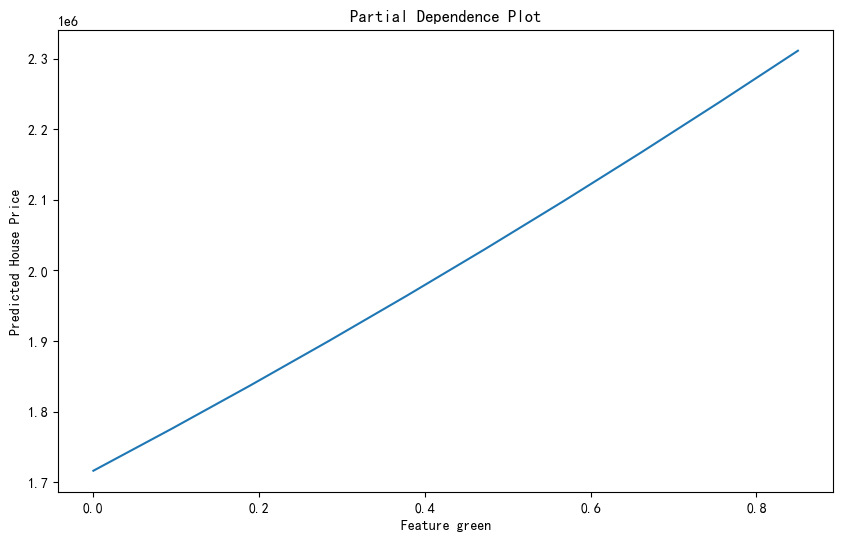
\includegraphics[width=\linewidth]{figure/pdp_green_train.png}
            \end{figure}
            \begin{figure}
                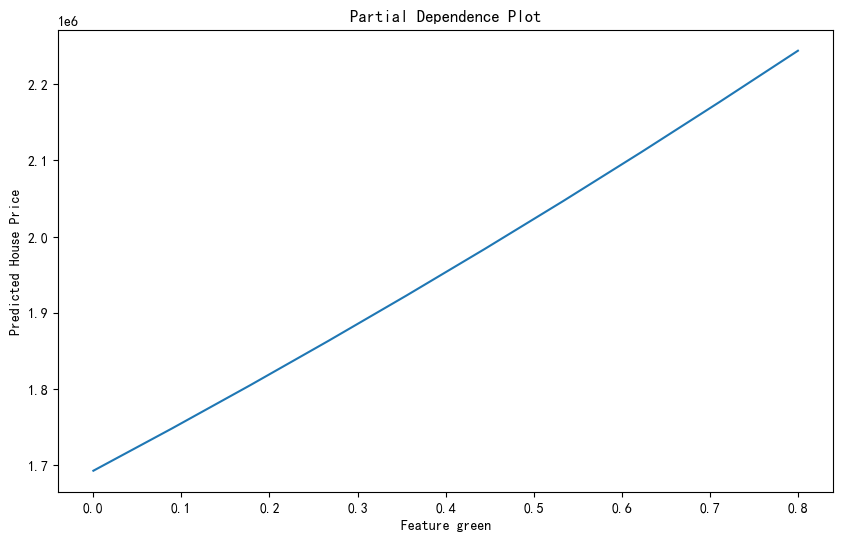
\includegraphics[width=\linewidth]{figure/pdp_green_val.png}
            \end{figure}
        \end{minipage}
        \begin{minipage}[t]{0.32\textwidth}
            \begin{figure}
                {\tiny 梯户比例}
                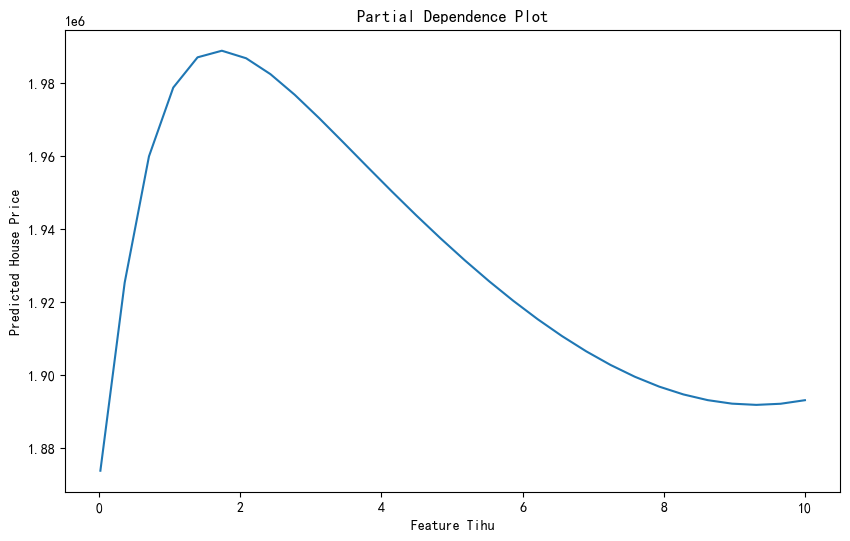
\includegraphics[width=\linewidth]{figure/pdp_tihu_train.png}
            \end{figure}
            \begin{figure}
                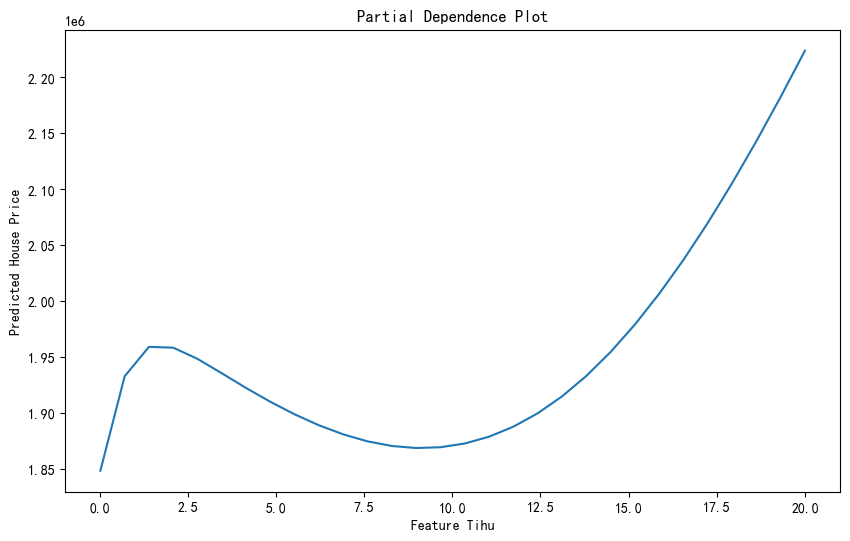
\includegraphics[width=\linewidth]{figure/pdp_tihu_val.png}
            \end{figure}
        \end{minipage}
    \begin{itemize}
        \small
        \item Ensemble model: OLS: XGB: ANN = 1: 0: 7.1 (Using Optuna)
        \item Insights: Community Name is (almost) all you need. Location information is the most important.
        \item Further exploration: (1)LLM? (2)ResNet? (3)coordinates(kNN)? (4)transaction time? (5)Macro features?
    \end{itemize}
\end{frame}

\end{document}